% !TeX spellcheck = cs_CZ
\begin{example}\label{fyz:fey_exam012}
  Dvě síly stejné velikosti \SI{250}{\newton} svírají úhel \ang{60}. Určete velikost výslednice.
      
  {\centering
   \captionsetup{type=figure}
   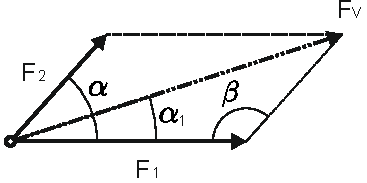
\includegraphics[width=0.5\linewidth]{fyz_fig380.pdf}
   \captionof{figure}{Grafické určení výslednice dvou sil se společným působištěm, svírajících 
     \(\alpha\). Také platí \(\beta = \ang{180}-\alpha\) a pak \(\cos\beta = - \cos\alpha_1\) 
   \label{fyz:fig380}}
  \par}
  
  Velikost síly \(F_v\) můžeme určit graficky pomocí vektorového rovnoběžníku. Velikosti sil 
  \(F_1\) a \(F_2\) vyneseme ve zvoleném měřítku (např. \SI{50}{\newton} = \SI{1}{\cm}), vykreslíme 
  rovnoběžník dle obrázku a délku uhlopříčku převedeme zpět ve stejném měřítku na velikost síly 
  \(F_v\). Početně určíme velikost výslednice pomocí kosinové věty: 
  \begin{align*}
     F_v^2 &= F_1^2 + F_2^2 - 2F_1F_2\cdot\cos\beta \\
     F_v^2 &= F_1^2 + F_2^2 - 2F_1F_2\cdot\cos(\ang{180}- \alpha) \\
     F_v   &= \sqrt{2F_1^2 - 2F_1^2\cdot\cos(\ang{180}- \alpha)}  \\
         &= \sqrt{2}F_1\sqrt{1-\cos(\ang{180}- \alpha)}         \\
         &= \sqrt{2}\cdot250\sqrt{1-\cos(\ang{180} - \ang{60})} 
            \cong \SI{433}{\newton}
  \end{align*}

\end{example}